\chapter{Modelling landscape evolution}
\label{chapter_landscape_evol}

\section{Introduction}
Landscape evolution models (LEMs) are quantitative tools used to simulate Earth surface processes and the evolution of the land surface. LEMs can be used to deduce whether hypotheses about landscape evolution are likely to be valid, by making quantitative predictions about their development. The earliest LEMs were conceptual and largely qualitative, such as the early pictorial landscape evolution diagrams by Gilbert (1880), Figure 1a. Gilbert’s model contains many of the key components in a modern LEM. The background schematic depicts the effect of an uplift field alone on the landscape, and the foreground depicts the combined effects of uplift and erosion. Gilbert also recognised the important concept of boundary conditions in LEMs, stating that the base of the diagram represents a fixed sea-level in this case.  These early models offered insight into the potential course of landscape evolution, and sowed the seeds for the later development of LEMs that abound today. In Figure 1b, a computer-based LEM (CHILD, Tucker et al. 2001) is shown, with the components of boundary conditions, uplift, and other process representations that are still core concepts in modern LEMs. The advent of computerised, numerical LEMs, such as those in Figure 1b, along with high-resolution digital topographic data provide important quantitative tools for investigating landscape process and form. 

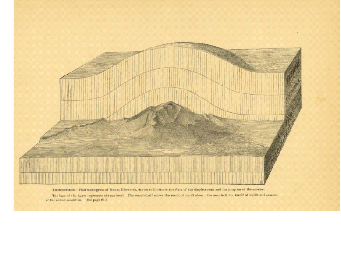
\includegraphics[width=7.86cm]{LEMFinalRevisedmanuscriptDAVFinalrevisions-img/LEMFinalRevisedmanuscriptDAVFinalrevisions-img001.png} 

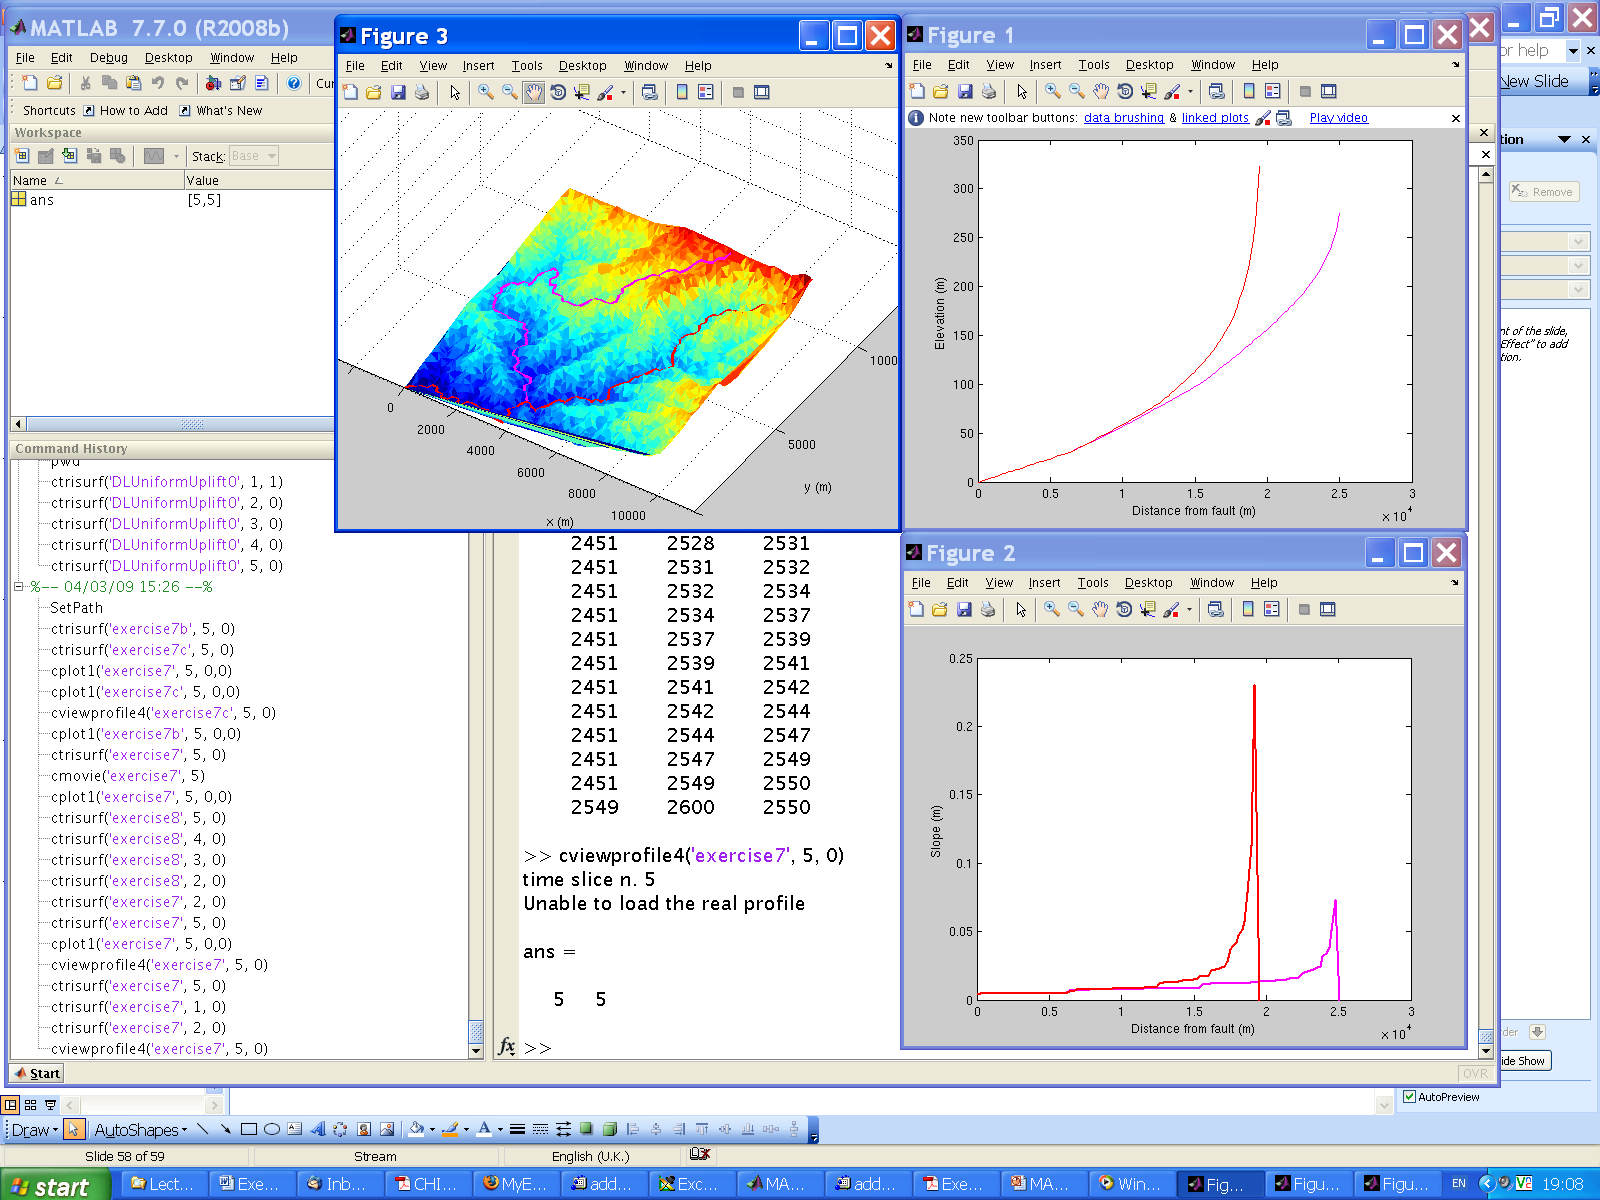
\includegraphics[width=7.883cm]{LEMFinalRevisedmanuscriptDAVFinalrevisions-img/LEMFinalRevisedmanuscriptDAVFinalrevisions-img002.png} 

Figure 1. The evolution of LEMs. (a) The diagrammatic LEM of Gilbert (1880) compared to (b) a computer numerical model (CHILD, Tucker et al. 2001). 

\subsection[Scope]{Scope}
This chapter provides a practical guide to the usage of numerical LEMs. Readers interested in more theoretical aspects of landscape evolution modelling should refer to other detailed literature reviews, such as those by Pazzaglia (2003), Martin and Church (2004), Willgoose (2005), Tucker and Hancock (2010), and Pelletier (2013). Other reviews focus on the use and application of LEMs, such as Van De Wiel et al. (2011); Willgoose and Hancock (2011); Temme et al. (2013). This chapter is not solely a software-type review of different LEMs (e.g. Coulthard, 2001), though comparisons between the features of various LEMs will be made to aid the prospective landscape evolution modeller. In short, the chapter aims to provide an overview of the usage, theoretical background, example applications, and software features of mainstream LEMs at the present time.

The application of physical analogue models is not discussed here, but readers can refer to Chapter 5.3 of this book: Green (2014). Numerical LEMs have not replaced their analogue counterparts – nor are they intended to. Physical models are actively used in landscape evolution studies (e.g. Hancock and Willgoose, 2002; Bonnet and Crave, 2006; Bonnet, 2009; Sweeney et al., 2015), but such experiments are usually custom-designed to meet the particular needs of a specific research question, and the materials available to construct the analogue model. In numerical landscape evolution modelling, there is more of a collective move (perhaps subconsciously) towards using a small number of community-developed numerical models, which are freely available to the modelling community.

The LEMs discussed in this chapter (see Appendix A) are primarily designed to simulate processes in humid–temperate sub-aerial environments. The role of glacial or aeolian processes are undoubtedly important in landscape evolution, but are frequently overlooked by the current range of available models. Glacial system modelling is covered in greater detail in Chapter 5.6.5 of this book (Rowan, 2011), and features discussion on LEMs that simulate glacial erosion processes (e.g. Braun et al., 1999; Egholm et al., 2011, 2012; Herman and Braun, 2008; Tomkin, 2007). Coastal, glacial, and aeolian processes are currently better catered for in environment-specific models (see the other sub-chapters in Part 5.6 of the book, Environment Specific Models, e.g. Rowan (2011), Grenfell (2015). However, the range of geomorphic process representation in LEMs continues to expand and develop.

\section{Fundamentals of Landscape Evolution Models}

\subsection{Governing Equations}

LEMs are ultimately driven by a set of mathematical equations – the geomorphic transport functions, often termed ‘laws’ (Dietrich et al., 2003; Tucker and Hancock, 2010). These laws may be derived from physical first principles, empirical evidence, or sometimes a combination of both. When implemented in a model, these laws are applied to a series of discretised cells or nodes representing the landscape. Conservation of mass is applied when calculating the fluxes in and out of neighbouring cells or nodes. (See Chapter 5.2 (Hutton, 2012) in this book for a more detailed description of mass continuity in numerical models.) The most common assumption made in most LEMs with respect to conservation of mass is that each column of rock or regolith has discrete boundaries between layers of different densities (Figure 2), i.e. there is no allowance for a dynamic variation of density throughout the each column in the model. Some models may further assume a uniform layer of substrate with no separate regolith layer. With these assumptions in mind, the majority of LEMs use a mass balance equation of the form:

\begin{equation*}
\frac{{\partial}\eta }{{\partial}t}=B-{\nabla}q_s
\end{equation*}
where $\eta $ is the surface elevation, t is time, B is a source such as the rate of sediment production, uplift or subsidence rate, and  ${\nabla}q_s$ is the divergence of flux of material – what comes in minus what goes out – in the x and y directions (after Tucker, 2010, eq. (3).) Further discussion of continuity of mass in LEMs can be found in Tucker (2010) and in Hutton (2012). 

\begin{figure}[t]
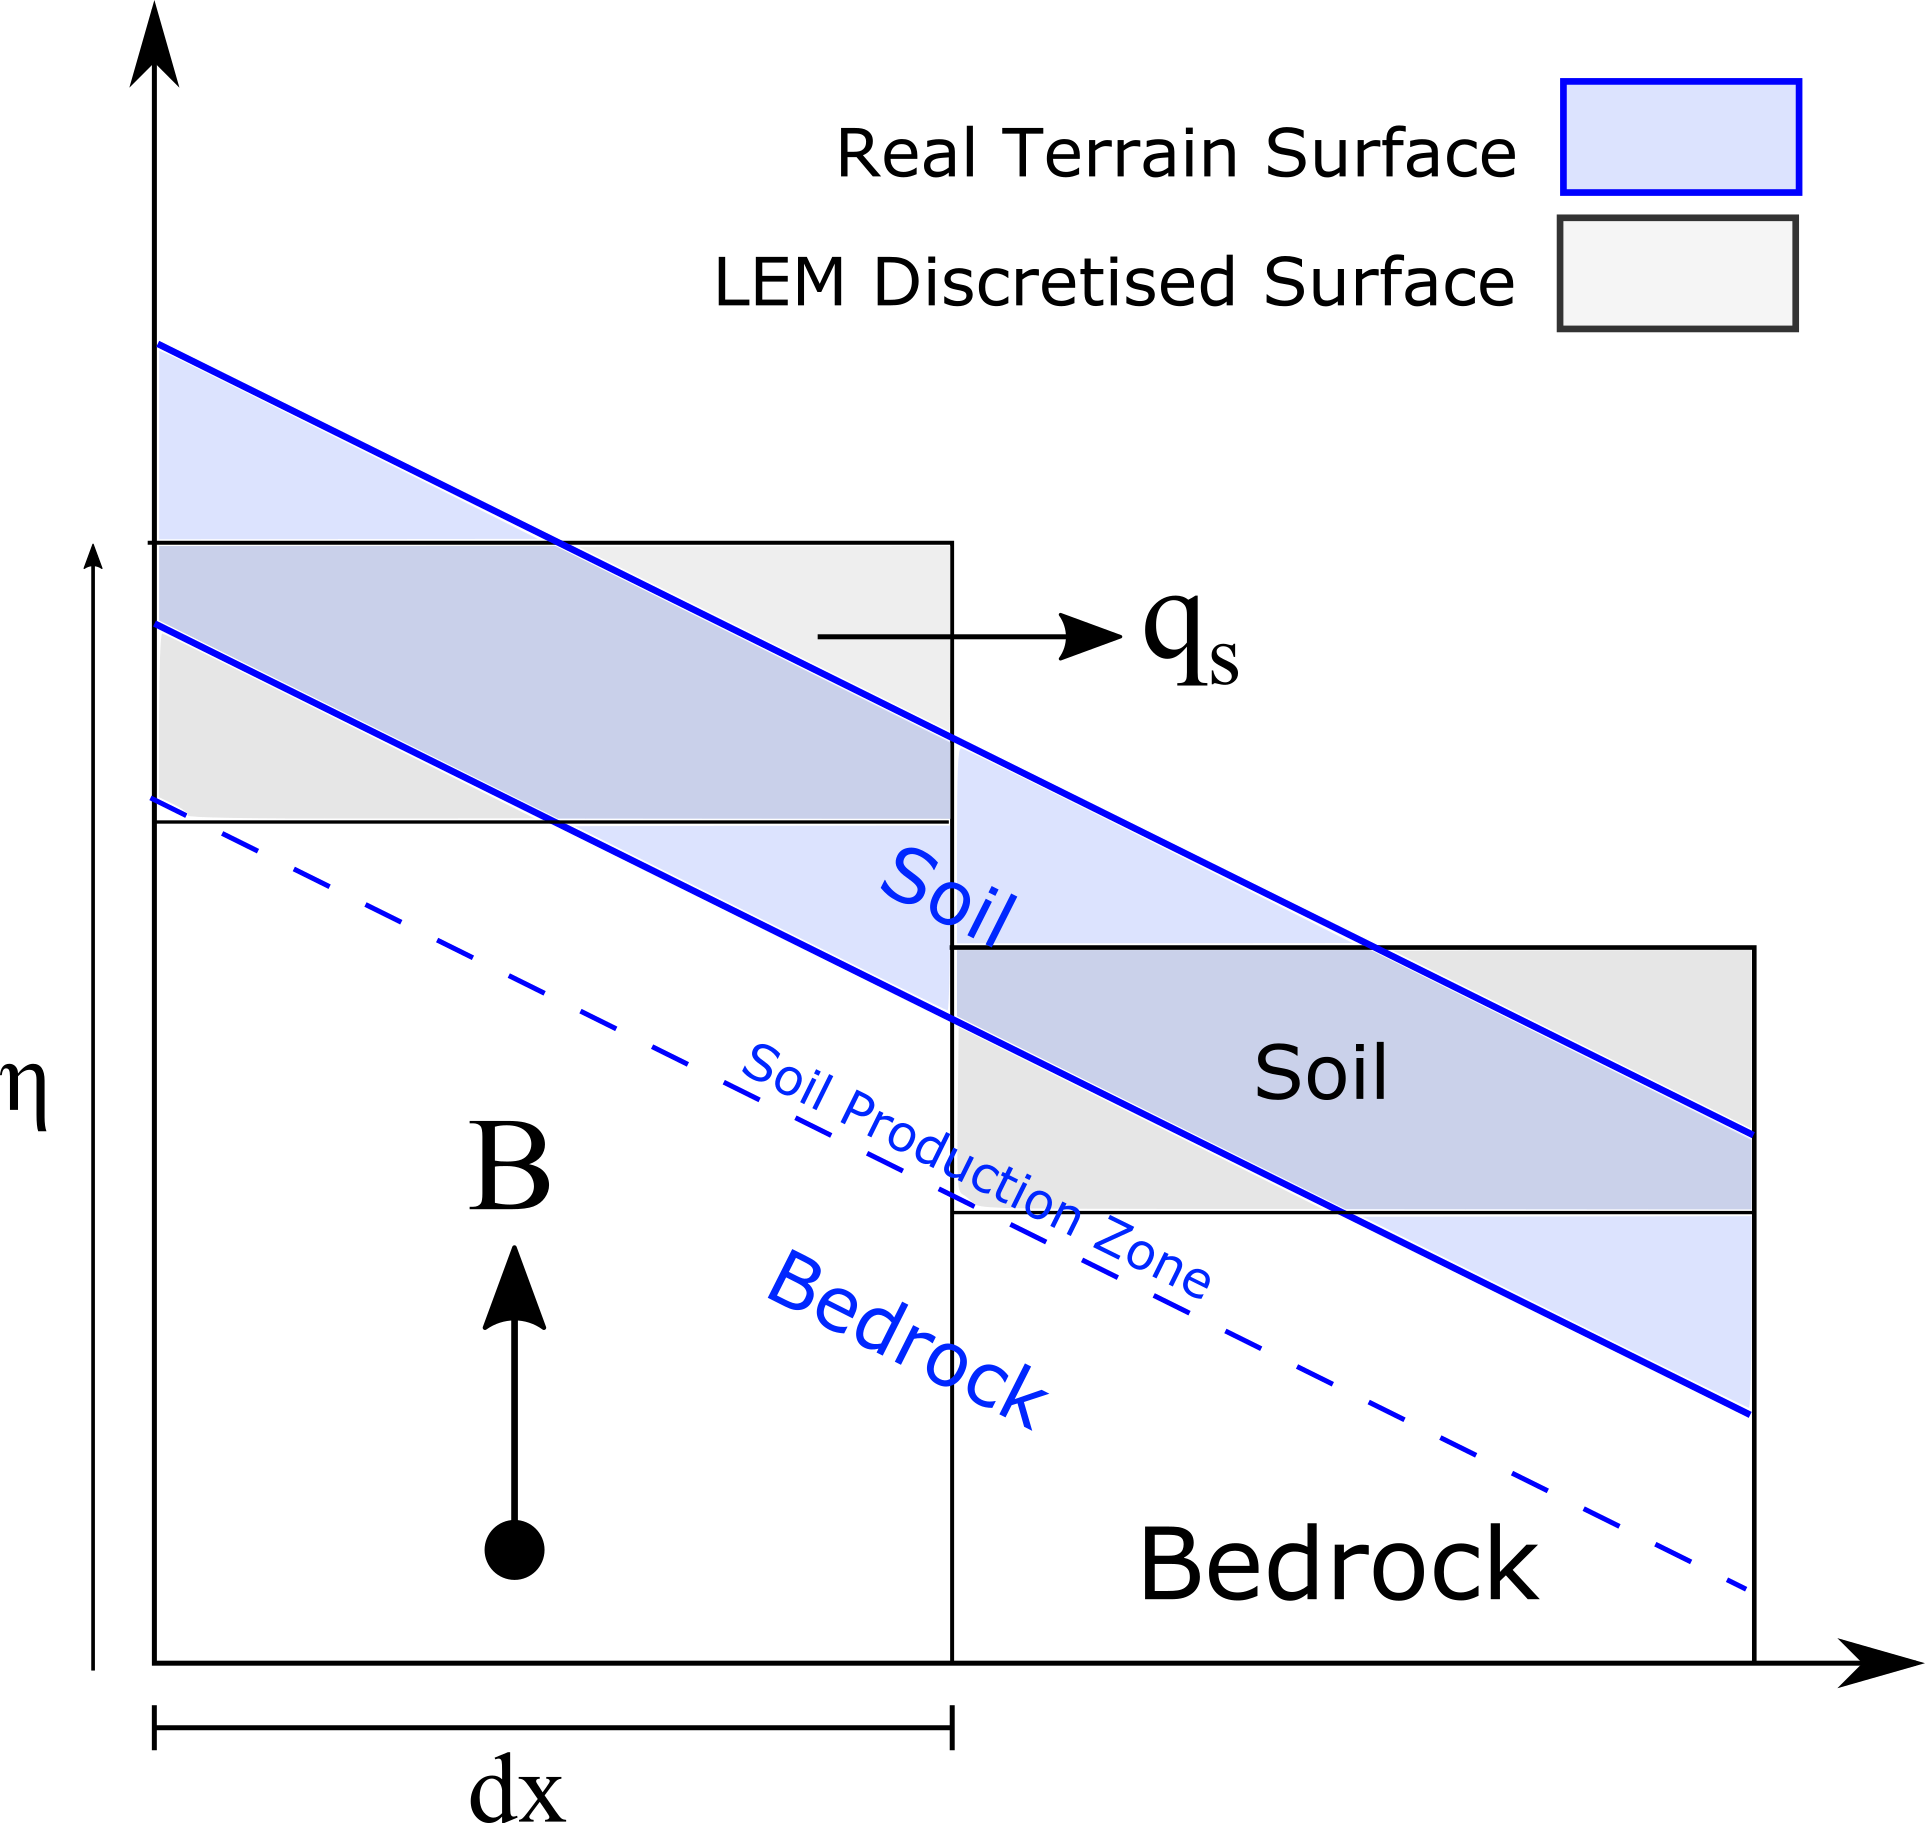
\includegraphics[width=11cm]{LEMFinalRevisedmanuscriptDAVFinalrevisions-img/LEMFinalRevisedmanuscriptDAVFinalrevisions-img003.png} 
\caption{Conservation of mass in a soil mantled landscape or sediment covered channel (after Dietrich et al., 2003; and Tucker, 2010). $\eta $ is the surface elevation, B is the boundary (base-level) change, qs the sediment transport term, and dx the grid cell size in a discretised landscape (assuming regular grid-spacing in this example).}
\label{fig_conservation_mass}
\end{figure}

The modeller must be aware of which equations are implemented in the chosen LEM. Simpler models may be based on a single equation for each process represented, or even a single geomorphic transport function representing bulk processes, such as the hillslope diffusion equation (Culling, 1960). More complex models offer the user a wide range of governing equations to select from – this allows comparisons to be made from using different theoretical models of sediment erosion and transport. The Channel-Hillslope Integrated Landscape Development (CHILD) model (Tucker et al., 2001b), for example, allows the user to select from several different governing equations for sediment transport, fluvial incision, and hillslope erosion.  

Each of these laws is based on a set of assumptions about the environments that they represent. The selection of the appropriate geomorphic transport law may be scale dependent. The basic stream power law, for example, does not scale well when applied to drainage basins below around 1 km2 in area (Hergarten et al., 2015; Stock and Dietrich, 2003). The LEM user should consult the appropriate literature to understand the basis limitations of specific geomorphic transport functions.

\subsection{Realism and Prediction}

An important question to ask in the selection of an LEM is what degree of physical realism is sufficient and appropriate for the hypothesis being tested. Models with a strong physical basis, for example those based on computational fluid dynamics (CFD) such as OpenFOAM (Jasak et al., 2007), or SPHysics (Gomez-Gesteira et al., 2012), may be appropriate for studying landscape evolution on very small scales, at the level where forces from multi-directional fluid flow and particle motion form part of the hypothesis (e.g. Bates and Lane, 1998; Jackson et al., 2015). The trade-off in using such models is the increased computational expense, which is why they are infrequently used in studies of landscape evolution beyond small scales.

Simpler representations of geomorphic processes in landscape evolution are often sufficient in lieu of fully physics-based models. Again, the appropriateness depends on the scale and complexity of the problem being studied. The value in using reduced-complexity models as exploratory tools is discussed in detail by Murray (2007). 

The question is often posed whether LEMs can be used as truly predictive tools (Hooke, 2003) to make quantitative, accurate, and confirmable predictions about how landscapes will respond to future environmental changes at human timescales (Pelletier et al., 2015). Recently, however, some authors have used LEMs to make quantitative forecasts about the evolution of landscapes in very specific environments, such as the response of coastal cliff erosion to climate change over the next century (Hackney et al., 2013), and the evolution and remediation of former quarries and tailings from mining operations (Hancock and Willgoose, 2004; Hancock et al., 2015b).

\section{Technical Implementation}
LEMs are designed to simulate the evolution of topography over a discretised x, y, z landscape surface, as shown in Figure 3. Usually this type of model is referred to as a 3D or ‘whole-landscape’ model (Willgoose, 2005). The term ‘2.5D’ is sometimes used as most LEMs do not explicitly use a vertical coordinate sensu stricto. Instead, the vertical dimension is modelled implicitly as a variable for each (x, y) grid cell. LEMs are implemented over a fixed spatial extent (the model domain), with pre-defined boundaries, as denoted by the x and y directions in Figure 3. 

\begin{figure}[t]
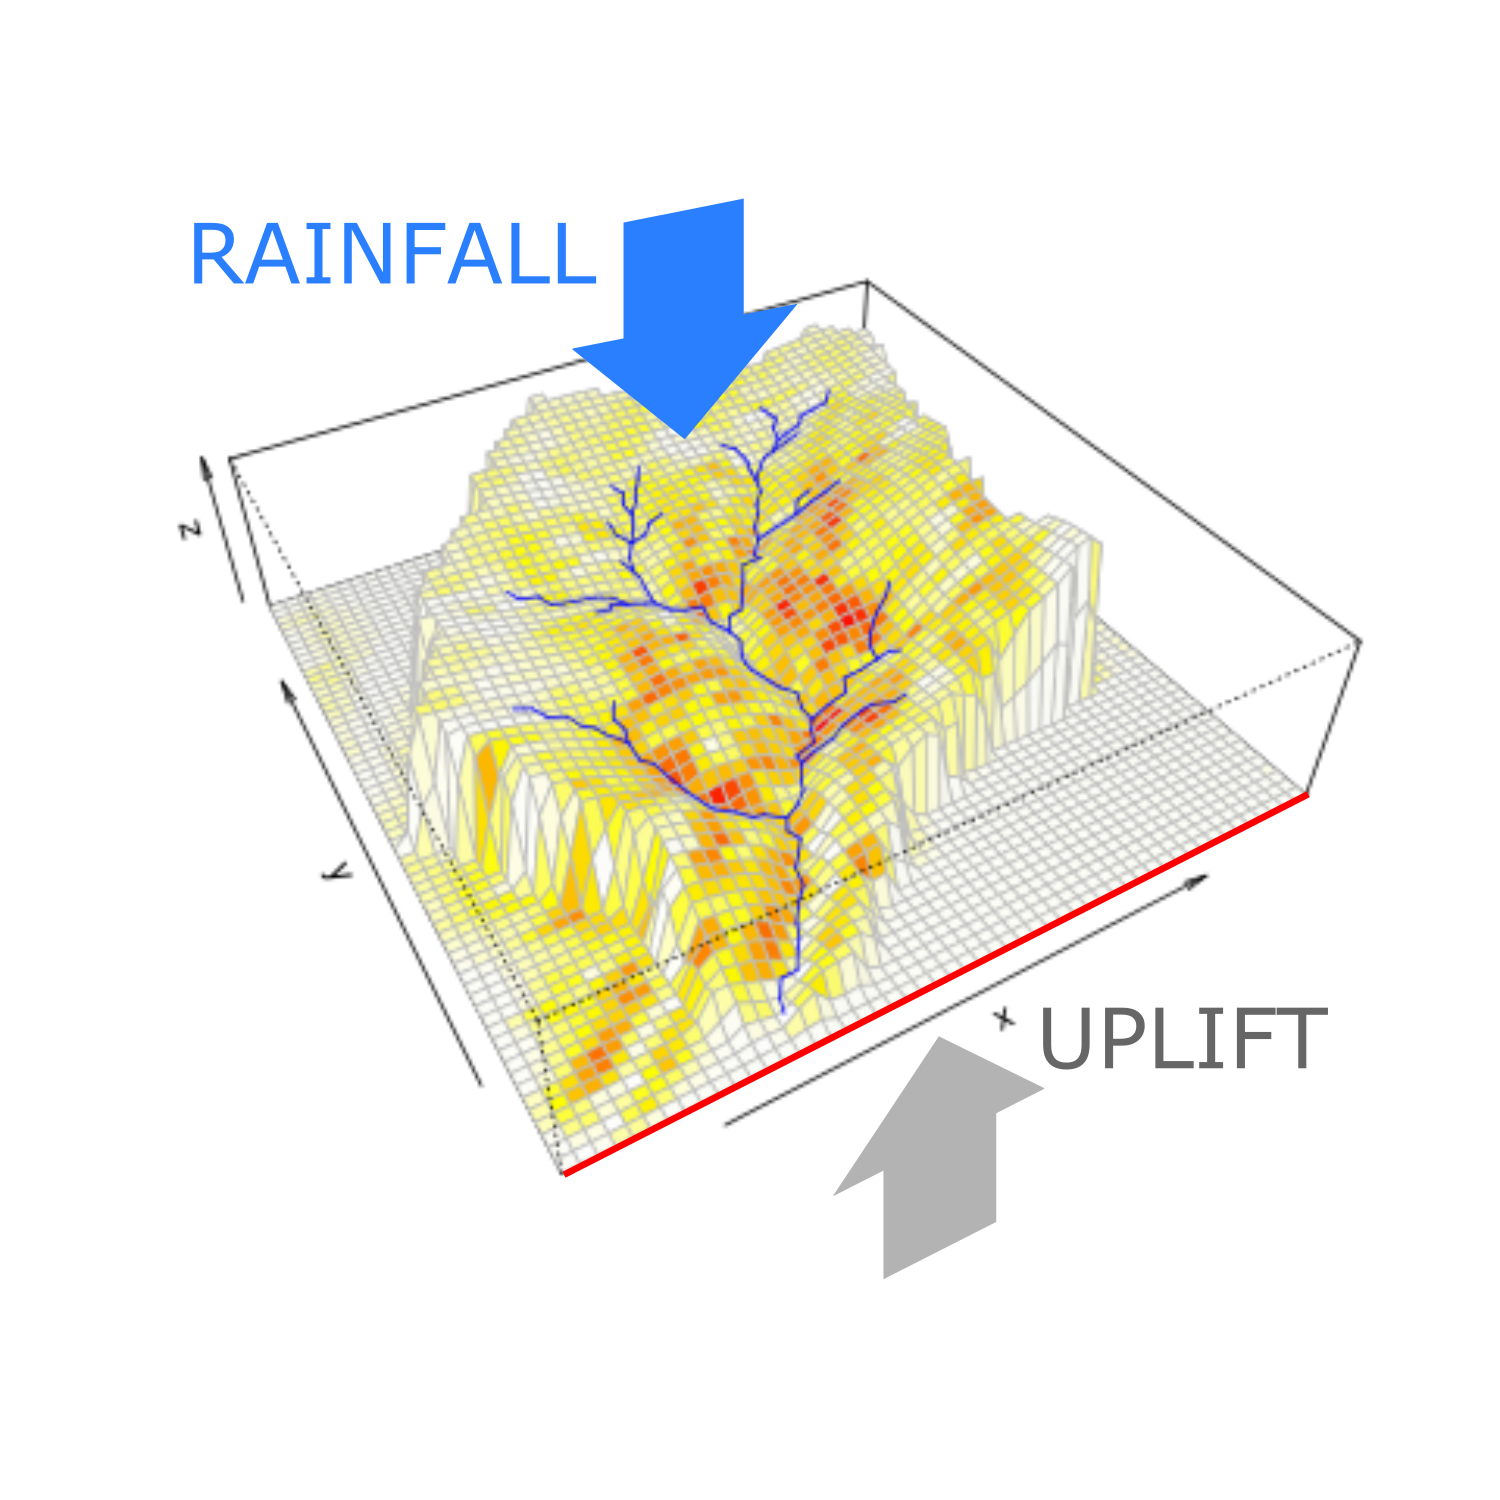
\includegraphics[width=11cm]{LEMFinalRevisedmanuscriptDAVFinalrevisions-img/LEMFinalRevisedmanuscriptDAVFinalrevisions-img004.png} 
\caption{Main components and boundary conditions of a landscape evolution model. Boundary conditions include the climatic, tectonic and base-level conditions (rainfall and uplift), as well as the conditions specified on the model domain edges, such as where water and sediment can leave the model domain (shown by the red line). Channel network shown by blue lines. Erosion rate (red-yellow) is shown as a grid cell variable in this example.}
\label{fig_main_LEM_components}
\end{figure}


\subsection{Grid and Discretisation}
The grid or mesh representing the land surface may be regular (rectilinear cells) or irregular, such as a triangular irregular network (TIN). The discretisation method of the terrain, and for rectilinear gridded domains the grid-cell size, dictates the length scale of landscape features that can be resolved in the model. Figure 4a depicts a typical regular gridded model domain. In this case, the maximum resolution of the river channel (in blue) is limited to the grid cell size of the model domain, or digital elevation model (DEM) used to initialise the model. Consideration should be given to whether the input data and model domain are of fine enough grid-spacing to resolve geomorphic features of interest.

\begin{figure}[t]
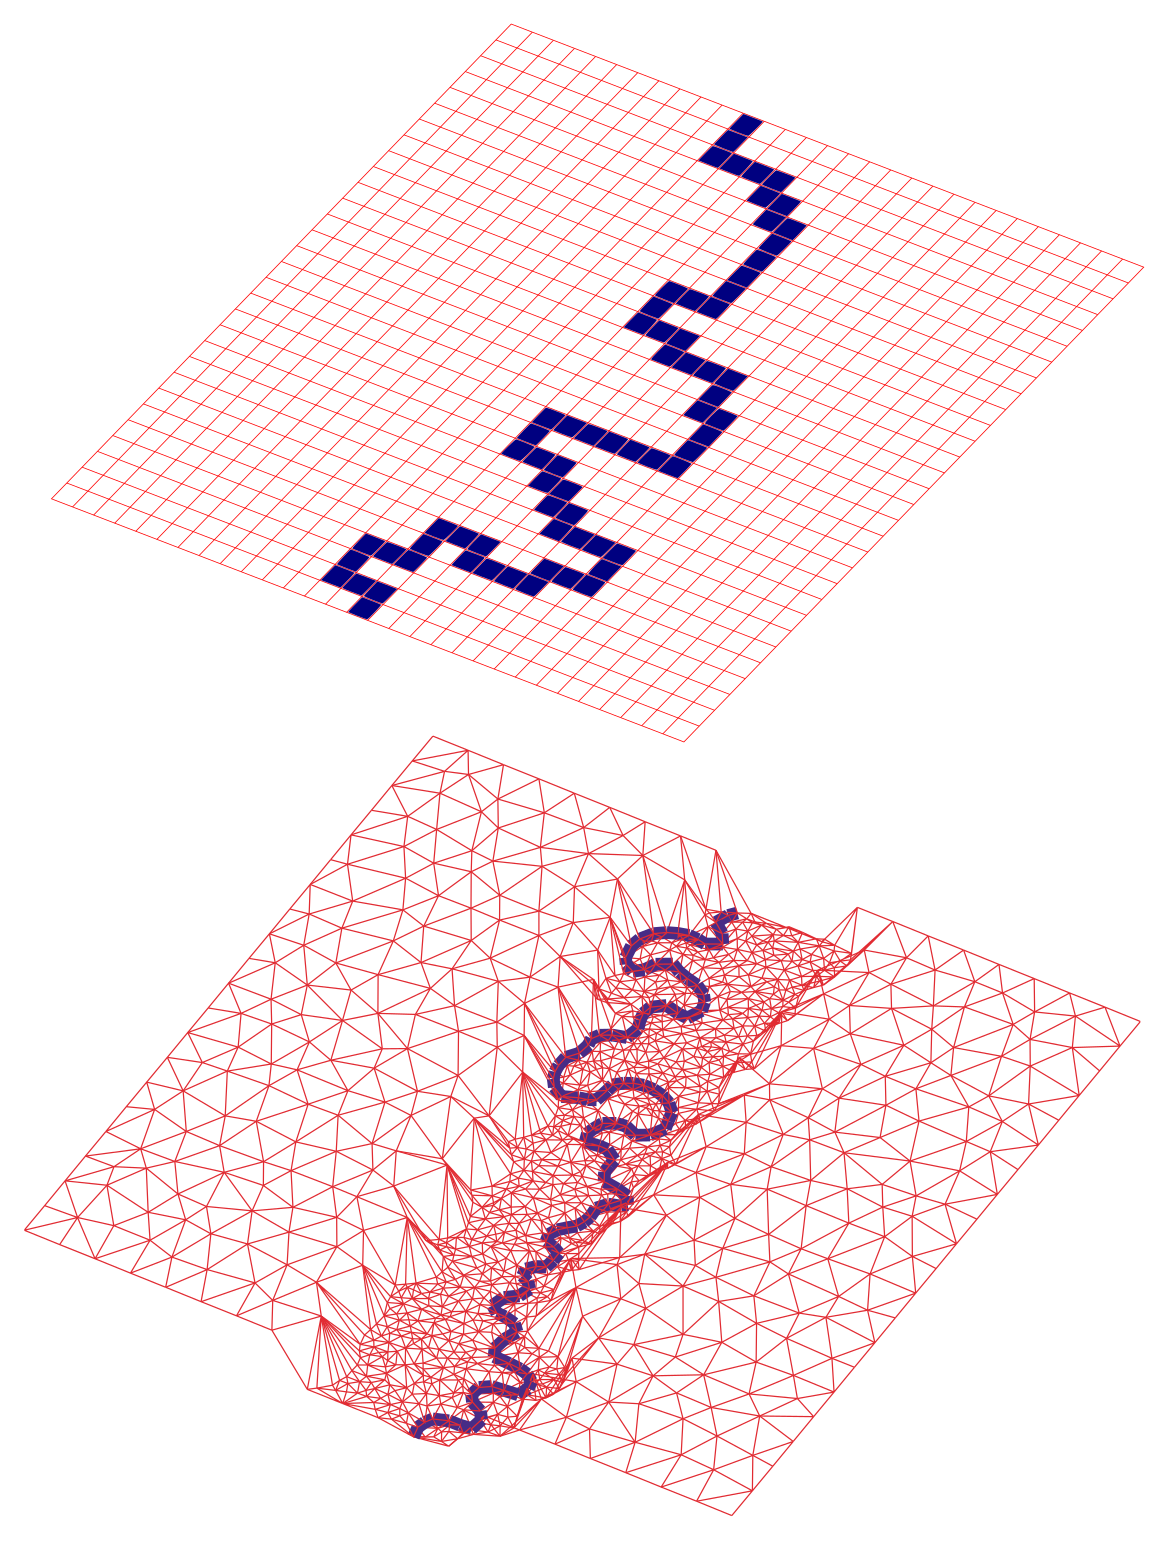
\includegraphics[width=11cm]{LEMFinalRevisedmanuscriptDAVFinalrevisions-img/LEMFinalRevisedmanuscriptDAVFinalrevisions-img005.png} 
\caption{A comparison of two terrain-discretisation approaches. a) Regular, rectangular gridded discretisation. b) TIN, (Triangulated Irregular Network), with adaptive re-meshing. (Figure 4b re-drawn from Tucker, et al. 2001b).}
\label{fig_LEM_discretisation}
\end{figure}

The advantage of irregular gridded models is that they allow adaptive re-meshing to finer grid-spacing (Figure 4b) where detailed resolution of certain geomorphic features is advantageous, such as in river channels or gullies (Braun and Sambridge, 1997; Tucker et al., 2001a). Triangular irregular networks also have advantages for the representation of drainage networks – flow routing is not restricted to 45 degree increments as it is in regular, square-gridded models (Figure 5) (Tucker et al., 2001b).

In regular gridded LEMs, the grid cell size is uniform across the entire model domain. Regular gridded models dominate the current range of models, being computationally less expensive, and having a source code structure that is often easier to understand, if modifications need to be made. Regular gridded models are more easily compatible with the common raster formats of DEMs, such as TIFF and ASCII raster data, as well as other data inputs derived from remote sensing such as land-use, soil moisture, and vegetation cover.

\subsection{Surface Flow Routing}
In real landscapes surface water may flow in multiple directions over terrain, but in LEMs flow direction is limited by a flow-routing algorithm and the discretisation scheme representing the land surface. The simplest square-gridded models route water from a single cell into one of either 4 or 8 adjacent cells, based on the path of steepest descent (Figure 5), known as the D4 or D8 algorithms (e.g. O’Callaghan and Mark, 1984). D8 algorithms, though simple, tend to be too convergent – resulting in a channel network with each stream the width of a single grid-cell (Wilson et al., 2008). More complex algorithms use a scheme where water can be routed in multiple flow directions (MFD) and the total water flux can be apportioned over multiple cells (Figure 5).  However, this class of algorithm tends to be overly dispersive in water flow routing (Wilson et al., 2008).  

\begin{figure}[t]
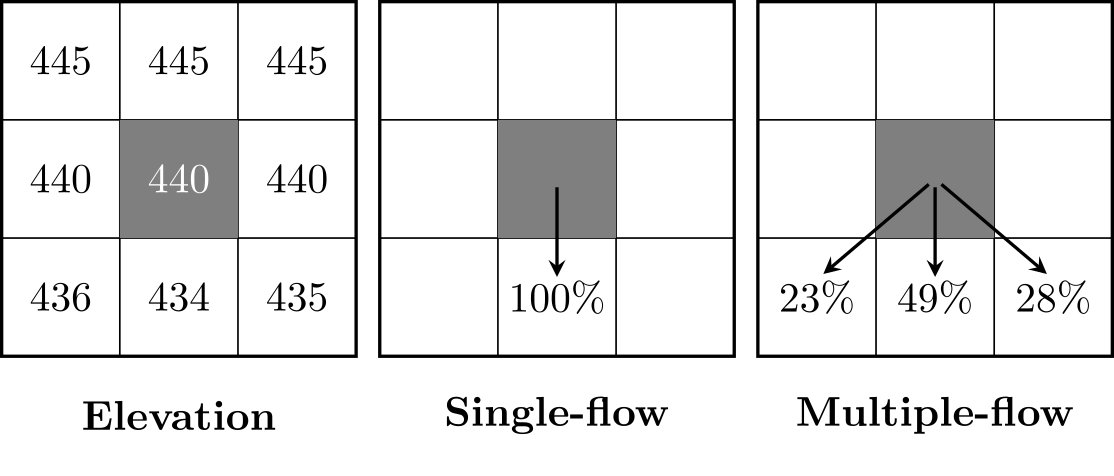
\includegraphics[width=11cm]{LEMFinalRevisedmanuscriptDAVFinalrevisions-img/LEMFinalRevisedmanuscriptDAVFinalrevisions-img006.png} 
\caption{Comparison of single- and multiple flow direction routing methods. (Re-drawn from Schäuble et al., 2008).}
\label{fig_LEM_flow_routing}
\end{figure}

The D-infinity scheme (Tarboton, 1997) is a single flow direction method aimed at addressing some of the limitations of the standard D8 algorithm. For detailed reviews of flow routing schemes see the works of Wilson et al. (2008) and (Schäuble et al., 2008). The appropriate scheme depends on the level of realism required for the hypothesis being tested. Simulations of complex riverine processes, incorporating braided channel networks, for example, would require a model with a multiple-direction flow-routing model.\- Flow routing models, with the notable exception of the FastScape algorithm (Braun and Willett, 2013), are typically the most computationally expensive part of a landscape evolution model, involving many iterative calculations per grid cell or node.

\subsection{Data Input Sources}

For modelling of real landscapes, thought must be given to the source data used to initialise the landscape surface in the model. In simulations of large-scale landscape evolution (model domains of tens to hundreds of kilometres), input data resolution can be relatively coarse, such as a 90m SRTM-derived (Shuttle Radar Topography Mission) DEM. Even this resolution may be higher than necessary and DEMs may be coarsened through resampling with GIS software in order to reduce the total number of grid cells and hence computational expense. Higher resolution DEMs are necessary for modelling small-scale features, such as gully formation or hillslope erosion (Nearing and Hairsine, 2010). It may be necessary to acquire sufficiently high resolution data, on the order of metres to centimetres, from sources such as airborne LiDAR (see Chapter 2.1.4, Gallay, 2013), terrestrial laser scanning (see Chapter 2.1.5., Smith, 2015), or structure from motion techniques (SfM, see Chapter 2.2.2, Micheletti et al., (2015). In short, the appropriate resolution of input data is dictated by the length scales at which the geomorphic processes of interest operate.

\subsection{Boundary Conditions}
Thought must also be given to the boundary conditions of the model domain. Boundary conditions refer to any input or constraint on the x, y, z minima and maxima of the model domain (Figure 3), including tectonic or base-level change, and climatic input, such as precipitation. Most models will operate on the principle of having at least one open boundary where water or sediment can flow out. In some models the placement of boundary outlets is customisable by the user (e.g. CHILD, FastScape). The LEM user should also consider the possibility that these boundary conditions may not be fixed over time, such as variation in rainfall rate or uplift rate. In some situations, the boundary conditions may exhibit some kind of feedback with the internal processes of the model domain (e.g. Raymo and Ruddiman, 1992; Willett, 1999).

\section{Current Models}

LEM development has bloomed in the previous two decades, in part due to significant and continued computational advancement, and there is now a wide variety of models to choose from. (See Appendix B for a systematic overview of the different LEMs available and their features and process representation). The range of models available vary in their complexity, applicability to different timescales, and different process representation. In this section, some of the existing LEMs currently in common use are briefly reviewed.

\subsection{CAESAR-Lisflood}

A family of related models have developed from the original CAESAR LEM (Coulthard et al., 1996, 2002). The original CAESAR model is a cellular automaton model that simulates water flow across the landscape, fluvial erosion, sediment deposition, and hillslope processes. CAESAR-Lisflood (Coulthard et al., 2013), the current iteration of the model, uses a more physical-based surface water flow component based on a simplified numerical solution to the shallow water equations (LISFLOOD-FP, Bates et al., 2010). The non-steady hydrological component of the model allows effects such as tidal flows, lake filling, and the blocking of valley floors by alluvial fans to be represented in LEMs (Coulthard et al., 2013). 

CAESAR-Lisflood is suited to simulation of entire drainage basins (in catchment mode) or sections of a river channel (in reach mode, e.g. Coulthard and van de Wiel, 2006; van de Wiel et al., 2007). CAESAR-Lisflood is an appropriate tool for timescales ranging from modelling the effects of a single storm over a few hours, through seasonal, to annual, and millennial time scales of landscape evolution. Process representation in CAESAR-Lisflood is focussed primarily on hydrodynamics and sediment transport, including the simulation of multiple-sized grain fractions. 

Though there is theoretically no upper limit to the time periods that can be simulated with CAESAR-Lisflood, existing studies have focused on shorter scales from decades up to thousands of years, such as simulating sediment output of a small basin under short term climate predictions (Coulthard et al., 2012a), simulating storm and tidal surge dynamics on coastal environments (Skinner et al., 2015), forecasting the short term geomorphic evolution of former mine-workings and excavations (Pasculli and Audisio, 2015), amongst others. 

\begin{figure}[t]
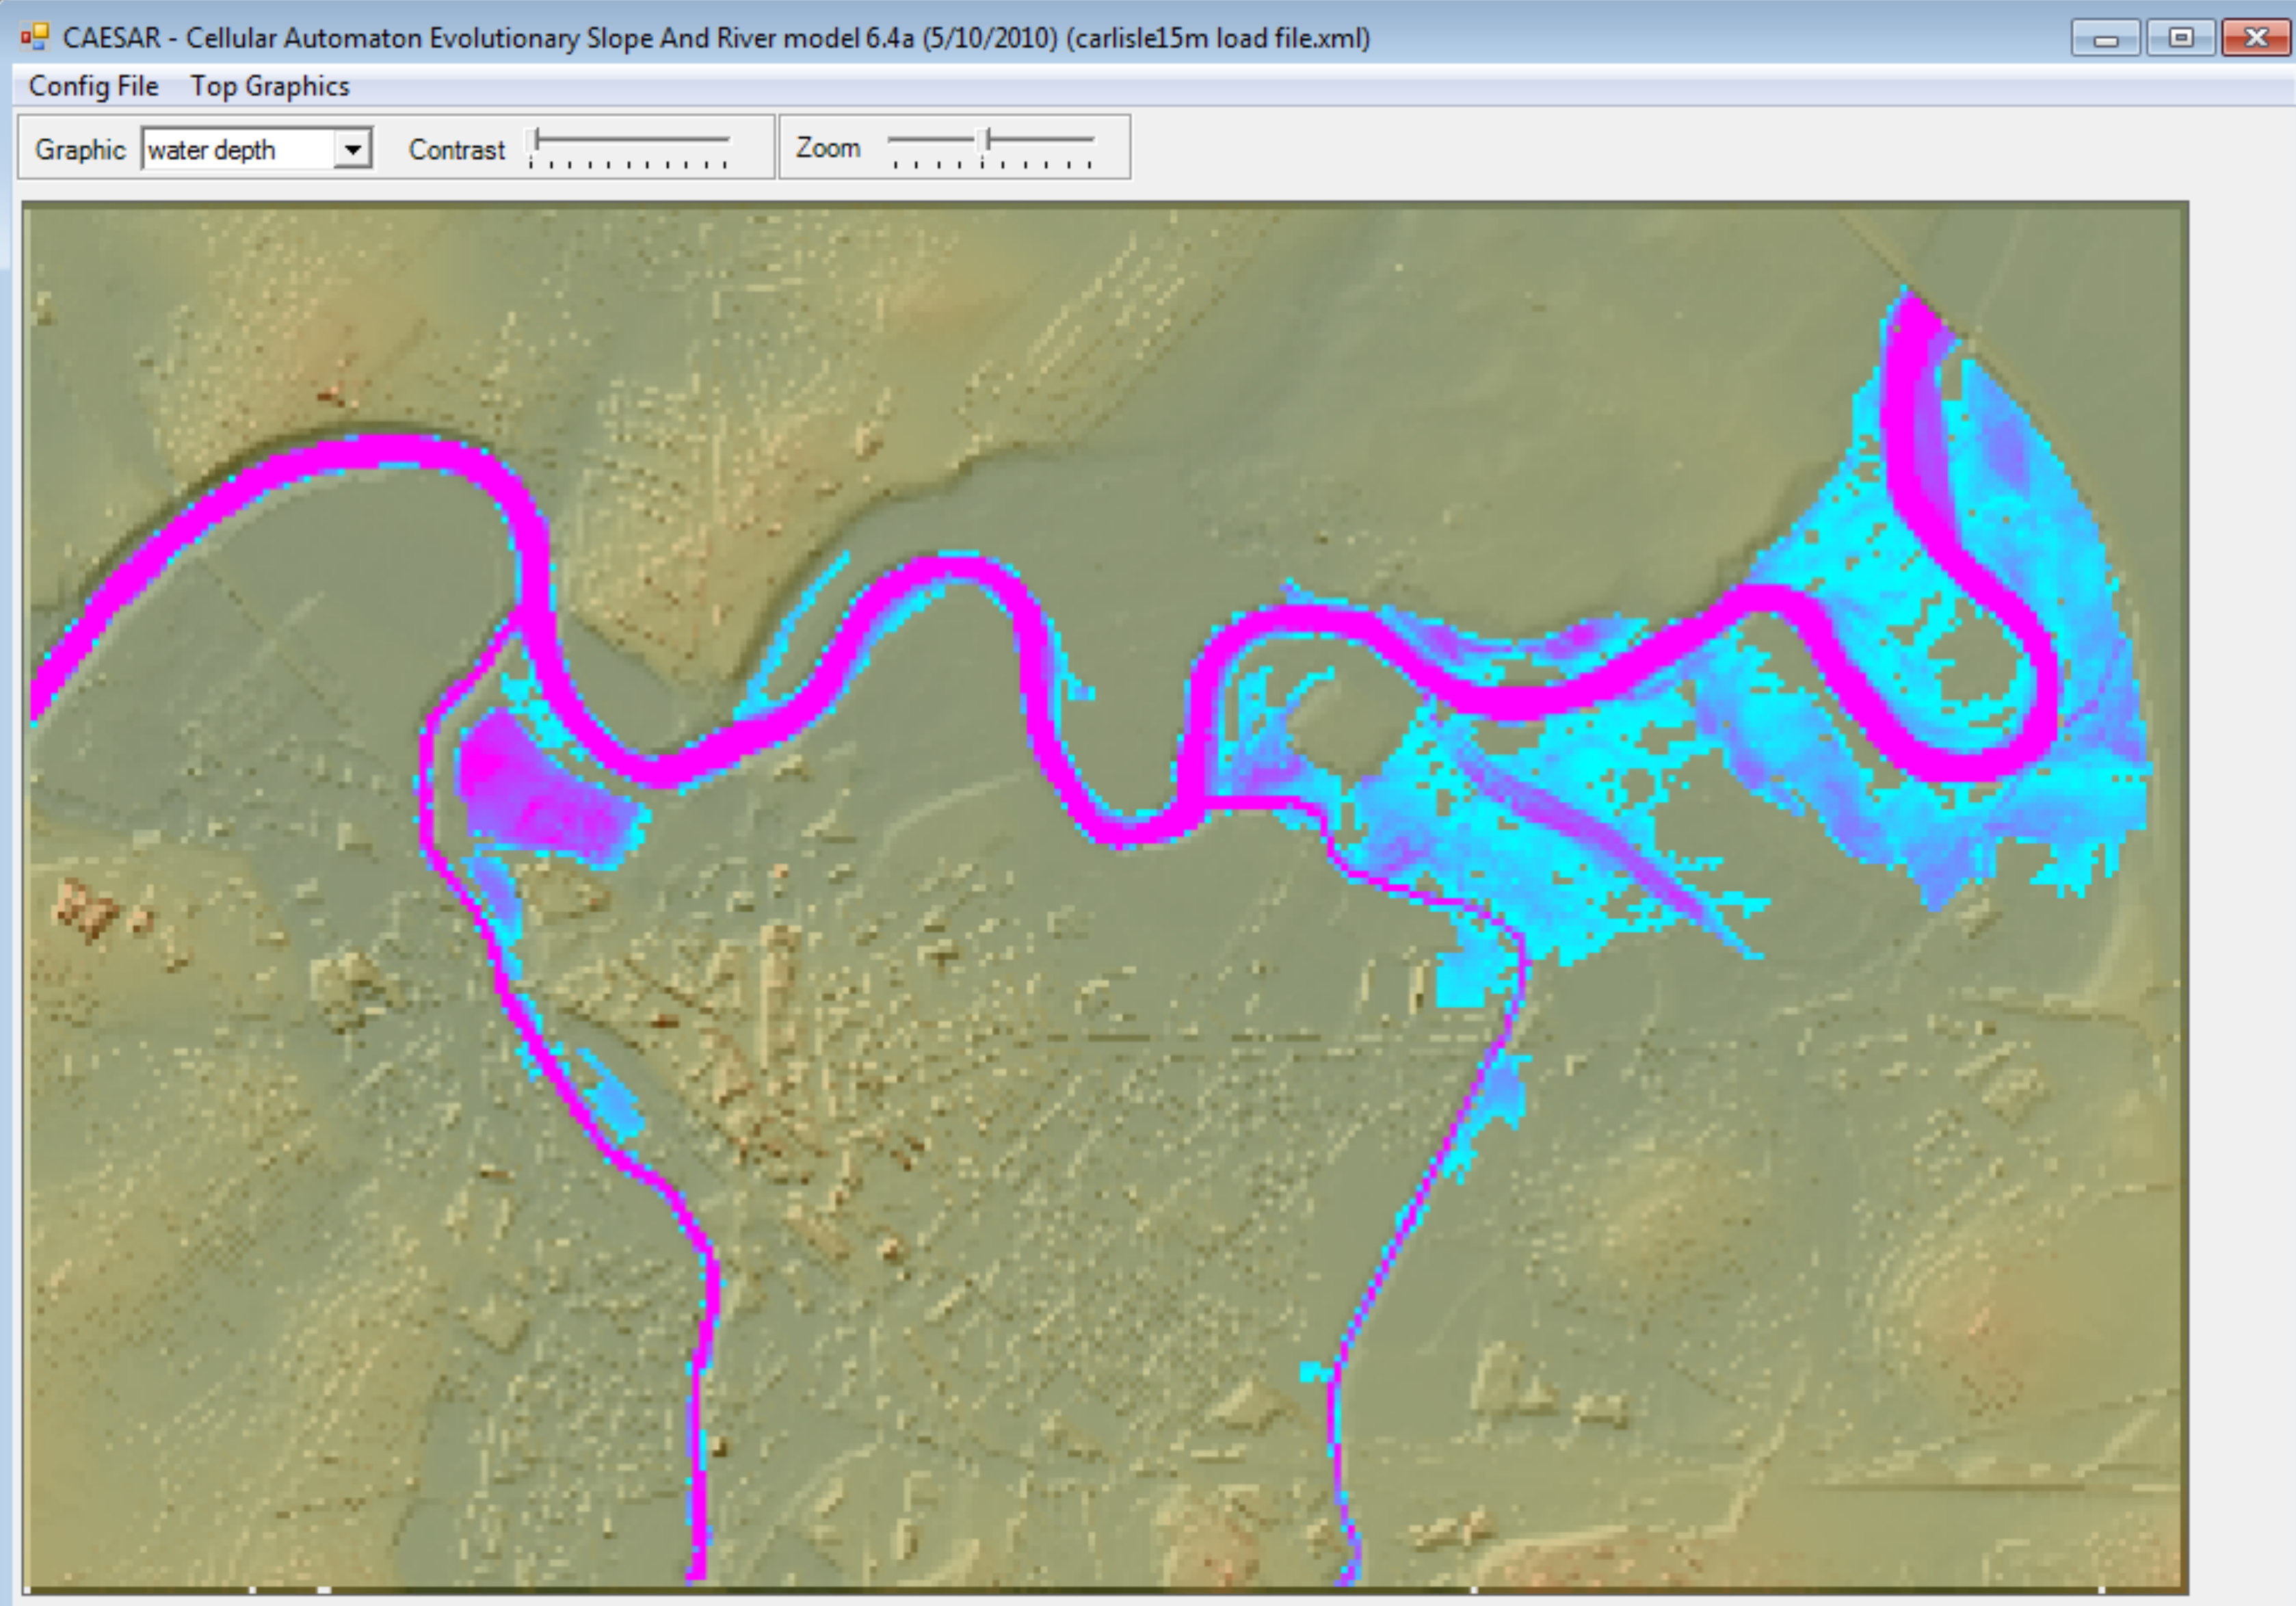
\includegraphics[width=11cm]{LEMFinalRevisedmanuscriptDAVFinalrevisions-img/LEMFinalRevisedmanuscriptDAVFinalrevisions-img007.png} 
\caption{CAESAR-Lisflood simulating the flooding of Carlisle, UK, 2005. Hydrogeomorphic effects of single floods can be simulated in this LEM due to the implementation of a non-steady flow hydrological component (Bates et al., 2010). Blue to pink colouring represents water depth, with pink indicating the deepest water depths. Model domain 5 km across.}
\label{fig_LEM_CAEASR_Lisflood}
\end{figure}

CAESAR-Lisflood uses a graphical user interface (GUI) to set model parameters and display output (Figure 6). The GUI makes model set-up quick and easier for users with less familiarity with command-line operations or code modification. The current version is limited to running in a Windows-only environment. The integration of visualisation with the core model code also allows the user to view model output as the simulation progresses (Figure 6), this has the advantage of letting the user monitor output without having to wait for a full simulation to complete and visualise the output in a separate step. 

\subsection{CHILD}

The Channel Hillslope Integrated Landscape Development model (CHILD, Tucker et al., 2001b) is another widely used model for investigating landscape evolution in a variety of environments, on temporal scales from decades to millions of years. The modular design of the LEM has facilitated its expansion over recent years and it now supports various types of geomorphic process representation. CHILD supports initialisation of the terrain surface from DEM data or generating synthetic topographies from scratch. A wide range of fluvial incision processes can be simulated with CHILD, including both detachment- and transport-limited erosion models, sediment transport, and a range of hydrological and rainfall-runoff generation routines. Recent development of modules has extended process representation to include, for example, modules of dynamic vegetation growth (Collins and Bras, 2004), floodplain evolution (Clevis et al., 2006), dynamic adjustment of channel width (Attal et al., 2008), representation of sediment grain size (Gasparini et al., 2004), debris flows (Lancaster et al., 2003), and stochastic rainfall generation (Tucker and Bras, 2000).

CHILD differs from many of the other models described in this section, as it eschews a traditional grid-based spatial discretisation in favour of a triangular mesh, or TIN. As previously discussed in the Technical Implementation section, this allows the model resolution to vary spatially across the domain, becoming higher in regions where smaller scale features and processes operate, such as river meanders, and coarser where features are much larger in spatial extent, such as floodplains and hillslopes (Tucker et al., 2001a). 

The CHILD model’s TIN-based approach is advantageous in its flexibility at representing different scale features within a landscape (Braun and Sambridge, 1997; Tucker et al., 2001b), but adds an extra layer of complexity when working with typical raster data formats, requiring conversion between raster and TIN data at the input and output stages of the modelling workflow. A series of MATLAB scripts are provided with the model for visualising output. The open-source RCHILD package is also available for output visualisation with the R programming language (Dietze, 2014). The CHILD model is platform-independent.

\subsection{FastScape-based LEMs}

FastScape is an algorithm based on an efficient implicit numerical scheme to solve variants of the stream power law for modelling large scale landscape evolution (Braun and Willett, 2013). The major advance made by the FastScape algorithm was to increase the efficiency of the flow routing calculation – a bottleneck in most LEMs – and hence the model is useful for rapidly testing hypotheses of landscape evolution. Several related LEMs have been based on an implementation of the FastScape algorithm, including:

\begin{itemize}
\item The ‘original’ FastScape LEM (Braun and Willett, 2013)
\item DAC – the Divide and Capture model (Castelltort et al., 2012; Goren et al., 2014)
\item LSDTopoTools: Raster Model (http://lsdtopotools.github.io, e.g. Mudd, 2016)
\end{itemize}
Recent applications of FastScape-based LEMs have focused on the simulation of synthetic landscapes under differing tectonic, lithological, and climatic boundary conditions (e.g Braun and Willett, 2013; Braun et al., 2014; Castelltort et al., 2012; Goren et al., 2014; Yang et al., 2015). The FastScape LEM also allows for the use of DEM data to set the initial surface topography in the model. An optional GUI interface is also included with the FastScape LEM, though this is currently only functional in Linux-based environments. The underlying FastScape algorithm is generic, and not necessarily tied to any particular LEM – users may choose to implement the algorithm in other open source models.

\subsection{LAPSUS}
The LAPSUS model (Landscape Modelling at Multi-dimensions and Scales) is a modular, multi-process model suited to studying catchment-scale erosional processes and landscape evolution at a range of temporal scales from years to hundreds of thousands of years  (van Gorp et al., 2015; Schoorl et al., 2000). LAPSUS is strongly suited to studying landscape evolution by means of soil and sediment redistribution through processes of fluvial erosion, surface wash, landsliding, tillage, creep, and tectonics. Applications include studying the interaction of non-linear processes in landscape evolution (Schoorl et al., 2014; Temme and Veldkamp, 2009), the role of tillage and changing land-use in decadal to millennial scale landscape evolution (Baartman et al., 2012b; Schoorl and Veldkamp, 2001), the sensitivity of soil erosion to rainfall intensity (Baartman et al., 2012a), and exploring uncertainty and parameter choice in landscape evolution modelling (Temme et al., 2011). LAPSUS features a graphical user interface similar in appearance to the CAESAR interface in Figure 6, allowing a similar visual monitoring of model outputs to take place without further post-processing required.  

\subsection{Other LEMs}

Landscape evolution modellers have a vast choice of models at their disposal: the organisation CSDMS (Community Surface Dynamics Modelling System:  http://csdms.colorado.edu) operates as a de facto model repository for developers and users of LEMs. The terrestrial model section lists well over one hundred different models that have been published to the site. CSDMS is a useful starting place for potential modellers to select an LEM based on their own requirements.  A summary of some of the more commonly used models over the last decade is presented in Appendix B, showing the key features of each model for comparison. 

Some LEMs extend the functionality (and often complexity) of existing models. For example, the CAESAR-Lisflood-DESC model (Barkwith et al., 2015) features, in addition to the core components of CAESAR-Lisflood, modules for distributed surface and soil hydrology, groundwater hydrology and a more physically realistic representation of landsliding. Applications of CLiDE have included the prediction of geomorphic and environmental hazards over human timescales (e.g. Barkwith et al., 2015; Tye et al., 2013). 

The current range of LEMs includes well established software packages such as the SIBERIA and CASCADE models. SIBERIA (Willgoose et al., 1991b) is a square gridded model originally developed to investigate the feedbacks between hydrology, catchment form, and tectonics (Willgoose et al., 1991a, 1994). CASCADE (Braun and Sambridge, 1997) was an early implementation of a TIN-based model designed to simulate long-term landscape evolution as a function of fluvial and hillslope processes.  Though the deployment of these two models has declined in recent years somewhat, they continue to be used as a benchmark in some studies (e.g. Hancock et al., 2015).

Recent developments within the modelling community have extended traditional modelling functionality with other elements of geomorphic analysis.  The LSDTopoTools software (http://lsdtopotools.github.io), for example, features an LEM based on the FastScape algorithm, integrated within a set of powerful topographic analysis tools. This allows easy transition between modelling and analysis of the results using common and novel topographic metrics. 

Another recent development is the Landlab software package (http://landlab.github.io/), which takes a highly modular approach to numerical modelling of landscapes. The user can rapidly create their own bespoke LEM from a set of existing components. This results in a high degree of user control over the complexity of the model configuration, not only in terms of process representation, but also the effect that technical aspects, such as grid type and flow routing algorithm have on model performance and output. The modular design avoids the usual expenditure of re-writing commonly used codes for process representation, model gridding, and standardised file input and output. A key strength of Landlab is its accessibility to users who do not have significant prior experience in designing and implementing numerical codes, but wish to embark on model development. Examples of Landlab’s applications include the study of impact cratering on landscape evolution (Hobley et al., 2013), the impacts of wildfires on hydrologic response (Adams et al., 2014), quantifying the link between regolith production and subsurface temperatures (Barnhart and Anderson, 2014), investigating the response of landscape evolution under non-steady state hydrology (Adams 2015), and as a basis for developing a stochastic cellular automaton model (Tucker et al., 2015).

The selection of LEMs discussed here range from those that have already established a wide user-base in landscape evolution research (e.g. CHILD, CAESAR, LAPSUS), to newer developments that offer novel functionality or process representation for modellers (e.g. Landlab, CLiDE, DAC, LSDTopoTools). Neither this section, nor the list in Appendix B is exhaustive, and some previously popular models have been omitted as it was felt they have been superseded or subsumed by newer offerings. The range of LEMs discussed here should nevertheless provide a starting point for tackling a wide range of modelling endeavours.

%\section{Applications and Examples}
%
%This section presents a short discussion of three recent studies using landscape evolution models. The selection was chosen to represent a broad selection of timescales, landscape types, and conceptual models. The reader should refer to the table in Appendix A for an expanded list of examples for further reading.
%
%\subsection[Testing Fluvial Erosion Laws (CHILD, Attal et al. 2008) ]{Testing Fluvial Erosion Laws (CHILD, Attal et al. 2008) }
%Several laws of fluvial erosion have been proposed to describe the evolution of river profiles (e.g. Seidl and Dietrich, 1992; Howard, 1994; Dietrich et al., 2003), and discriminating between which law is appropriate for a given landscape is challenging. Attal et al. (2008) tackle this by selecting river basins believed to be undergoing a transient response to base level change along an active fault (setting depicted in Figure 7). They use an LEM to test two of the common end-member models of fluvial incision: a transport-limited and detachment-limited case. The underlying process models are parameterised and calibrated using field data collected from the basins. Starting from a steady-state form of each basin’s topography, the CHILD model simulations are run with fault throw accelerations programmed at known intervals, which are well documented from previous studies.
%
%An inverse problem is set up, using an ensemble of model simulations to determine which combination of fluvial incision model and parameters produce the closest match to the observed topography. The study also benefits from careful selection of field sites with uniform lithologies, which helps constrain the range of variables. 
%
% 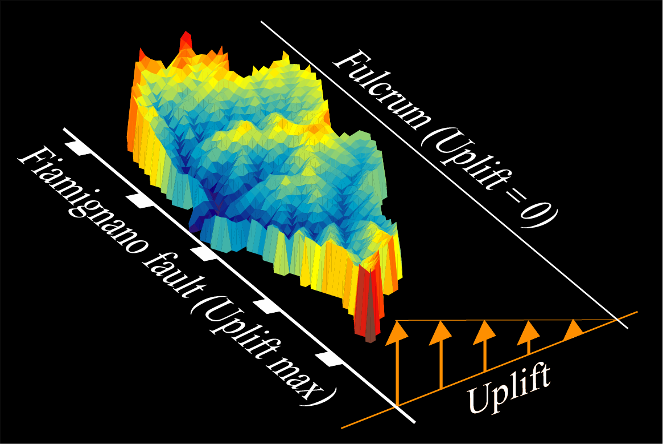
\includegraphics[width=7.883cm,height=5.272cm]{LEMFinalRevisedmanuscriptDAVFinalrevisions-img/LEMFinalRevisedmanuscriptDAVFinalrevisions-img008.png} 
%
%Figure 7. Example output from the CHILD model used in Attal et al. (2008). Landscape response to tectonic perturbation (fault throw acceleration) is shown. Example using real topography in the Italian Apennines. 
%
%\subsection{Climate, Tectonics or Morphology in Sediment Yields (CAESAR, Coulthard and Van De Wiel, 2013) }
%Landscape evolution covers a range of temporal scales – this study by Coulthard and Van De Wiel (2013) focuses on landscape evolution over short time periods of c. 100–1000 years. The study uses a forward modelling approach to predict the relative importance of different perturbations to a river catchment of approximately 500 km2 in the North of England. The CAESAR model was set up to run a series of 100 year and 1000 year experiments, each with a single different tectonic or climatic perturbation introduced to each experiment, with all other conditions remaining the same.
%
%From the results of the experiments, the authors are able to predict the relative impacts of climatic versus tectonic perturbations on the catchment. For a transport-limited environment, the authors discover climatic changes have the greater effect on sediment yields at shorter timescales, with sediment signals from increased rates of uplift being lost in the internal storage of the basin. 
%
%The study shows that LEMs may be used to make useful predictions about sediment yields in order to assess the relative importance of external perturbations, rather than to precisely predict the amounts of sediment output. Furthermore, landscape evolution is the result of a complex interaction of several competing processes, and by carefully isolating each process or potential perturbation in separate experiments, it is possible to explore which factors have the most significant impact on drainage basin evolution.
%
%\subsection{Coupled Numerical-Analytical Approach to Landscape Evolution Modelling (DAC-FastScape, Goren et al. 2014) }
%This study tackles a shortcoming in previous LEMs where the form and processes associated with drainage divides were under- represented in models, and investigates the implications on landscape evolution at the range scale, with an LEM that can accurately represent drainage divides. The authors propose a hybrid numerical-analytical model called ‘Divide and Capture’ (DAC, based on the FastScape algorithm of Braun and Willet, 2013), which calculates the positioning of drainage divides based on a sub-grid scale parametrisation of divide migration. Their precise analytical description of water divides is found to alter the dynamics of basins either side of the divide. Using a synthetic landscape (Figure 8), they find that the time taken for landscapes to reach steady state is longer due to the dynamic reorganisation and basin capture that persists about drainage divides, long after traditional LEMs would have reached steady state. 
%
%The study tackles the problem using a range of synthetic topographies, and is an example of using LEMs in an exploratory way to make general predictions about landscape form. The latter half of the study shows that ‘real’ topographies can be simulated in general terms, using a model set-up that simulates the key features of the New Zealand Southern Alps. A real DEM is not used, but by carefully choosing the initial conditions, parameters, and tectonic boundary conditions the authors show that this simplified version of a landscape is sufficient to represent the key characteristics of their study area (Figure 8).
%
%\begin{figure*}[htp]
%\centering
%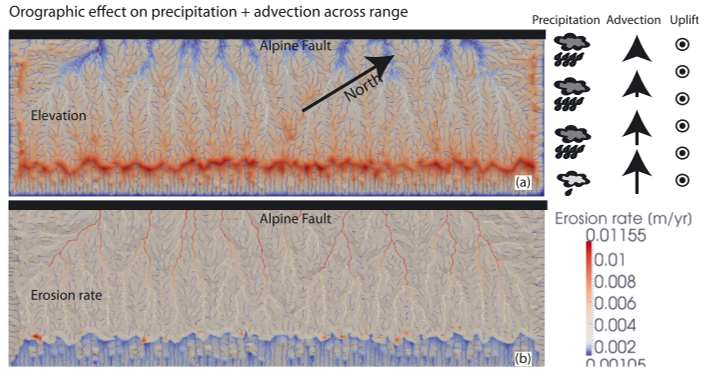
\includegraphics[width=16.854cm,height=4.812cm]{LEMFinalRevisedmanuscriptDAVFinalrevisions-img/LEMFinalRevisedmanuscriptDAVFinalrevisions-img009.png}
%\end{figure*}

\section{Uncertainty, Sensitivity, and Calibration}

\subsection{Uncertainty}
Uncertainty in modelling describes our inability to know precisely the initial conditions of a model, to represent in a model all the processes that govern landscape evolution, and ultimately to know with certainty the accuracy of the predicted outcome (Beven, 1996; Pelletier et al., 2015). All LEMs make simplifications regarding process representation, partly due to a lack of detailed knowledge in how certain processes work, and partly due to limitations about how these processes can be represented in computer models.  Uncertainty may also stem from inaccuracies in input data sources, the choice of model parameters, and the boundary conditions of the model (and whether these parameters and boundary conditions might change through time). Uncertainty in LEMs may lead to errors that propagate through the simulation and increase in magnitude as a simulation progresses. 

Ideally, one should address uncertainty by first assessing which parameters the model is most sensitive to – it may be that large uncertainties in one parameter have relatively little effect on the model outcome, whereas small uncertainties in a different parameter produce unexpectedly large variation in the model outcome (Pelletier et al., 2015).

Methods such as ensemble analysis should be considered, whereby multiple instances of the same simulation are run, with a range of parameters chosen from a probability distribution to assess the most likely outcomes from a model. While uncertainty cannot be removed entirely from modelling studies, it is useful to be able to state the most probable outcome(s), based on a probabilistic distribution of input conditions.

Uncertainty is a particular challenge in landscape evolution modelling as many processes are threshold dependent, or scale non-linearly (Schumm, 1979). In choosing parameter values, guidance should be taken from reported values of such parameters in the published literature. Readers are referred to Chapter 5.2, Numerical Modelling, (Hutton, 2012) for further discussion of uncertainty, as well as the review by (Pelletier et al., 2015), and LEM studies that have explored uncertainty in more detail (Hancock et al., 2015a; Mudd et al., 2014; Temme et al., 2011).

\subsection{Sensitivity and Calibration}
Following earlier definitions, (Oreskes et al., 1994; Trucano and Swiler, 2006) calibration is defined here as the selection and modification of input parameters of a model in order that they maximise agreement with observed data in real landscapes. Such parameters in LEMs might include the coefficient terms in fluvial erosion laws, for example the K, m, and n parameters in the stream power law (Seidl and Dietrich, 1992), hydrological parameters such as Manning’s n (Manning et al., 1890), or the threshold shear stresses required to initiate erosion (Snyder et al., 2003). Many such parameters are not directly quantifiable by field measurement, and model users should consult similar studies for recommended values, or conduct their own sensitivity analyses to constrain uncertainty in parameter choice. Other parameters may lend themselves to more rigorous methods of calibration, where they link directly or indirectly to measurable values in the field. Examples would include the calibration of hydrological parameters to produce a ‘best fit’ with observed discharge values at river gauging stations (e.g. Coulthard et al., 2013; Wong et al., 2015), constraining stream power law parameters using statistical models and sensitivity analyses (Croissant and Braun, 2014; Mudd et al., 2014), or the field measurement of sediment shear strength to assist in setting erosion threshold parameters (see Chapter 1.3.1, Grabowski, 2014).

\section{Validation \& Confirmation}
Validation is the process of assessing the legitimacy of a model set-up. Results from a model may or may not be valid depending on the quality of input data and model parameter choice (Oreskes et al., 1994). Moreover, (as noted by Oreskes et al., 1994) validation does not necessarily establish the truth or accuracy of model predictions, only that the model is internally consistent. In practice, it can be thought of as a ‘sanity check’ on the input to the LEM before beginning the simulation. For example, is the input DEM of sufficient resolution to represent the scale of geomorphic features expected to be formed? Do the input parameters conform to observed or realistic ranges? (See Calibration in previous section). If the answers to these types of question are ‘no’, the model predictions will be invalid. 

Geomorphologists use LEMs to deduce whether hypotheses about landscape evolution are likely to be valid, which requires a method for assessing how the model output supports the hypothesis. Confirmation refers to the assessment of how model predictions – after selecting suitable input parameters – match observations in nature (Oreskes et al., 1994). Directly observing landscape evolution is challenging at human timescales, as whole-landscape change occurs at slow pace, making direct confirmation of model predictions difficult in many situations (Hasbargen and Paola, 2003; Hoey et al., 2003). Some predictions made by LEMs, however, can be directly or indirectly confirmed to a certain extent with field observations. This includes short term phenomena such as gully formation, coastal erosion, and river bank incision. At short timescales, direct monitoring and quantification of erosion rates, particularly in rapidly eroding fluvial settings, becomes feasible. 

\subsection{Field Confirmation}
Techniques to indirectly measure the rates of landscape change are wide-ranging, and include measuring sediment flux at catchment outlets, using traps to measure bedload erosion and deposition (e.g. Bunte et al., 2004), bedload impact sensors (e.g. Raven et al., 2010; Rickenmann and McArdell, 2007; Turowski et al., 2010), suspended sediment measurements at gauging stations (Brazier, 2004), and the use of radio frequency identification-tagged sediment particles to track sediment movement (e.g. Beer et al., 2015; Chapuis et al., 2015). Further information on such measurement techniques can be found in Parts 3.3 (fluvial) and 3.4 (glacial) of this book. 

Through the rise of digital photogrammetric techniques, such as airborne and terrestrial laser scanning, direct measurement of whole-landscape morphological change is now possible at high enough resolutions to quantify small differences in topographic features, particularly in rapidly evolving landscapes (e.g. Rosser et al., 2005; Vaaja et al., 2011). Using these methods to aid model confirmation would be limited to small scale studies, as processing of point cloud data from these sources can be highly computationally expensive (Axelsson, 1999). Parts 2.1 (Direct acquisition of elevation data) and 2.2 (Photogrammetric techniques) provide more information on related measurement techniques. Chapter 2.3.2 (Williams, 2012) covers the use of DEMs of difference to quantify landscape change over discrete time periods. Despite their availability, there are as of yet few examples that employ these direct methods of landscape quantification in the confirmation of predictions made by LEMs.

At longer, geomorphologically significant timescales, a range of techniques becomes available to assist in the calibration of LEMs and confirmation of hypotheses. Two popular techniques are mentioned here, but other suitable techniques may be found in relevant reviews and textbooks (e.g. Anderson and Anderson, 2010; Burbank and Anderson, 2011). 

Optically stimulated luminescence dating uses a property of quartz and feldspar minerals that records the amount of time they have sat in a sedimentary or soil deposit, which can be used for dating landforms (Aitken, 1998; Murray and Wintle, 2000; Stokes and Clark, 1999). The applicability of this technique to different temporal scales is site-specific and ranges from years to upwards of hundreds of thousands of years (Madsen and Murray, 2009). A more comprehensive overview is provided in Chapter 4.2.6 of this book (Mellett, 2013).

Cosmogenic radionuclide (CRN) dating is a technique based on the interaction of cosmic rays with certain isotopes in minerals in the Earth’s surface (Anderson et al., 1996; Dunai, 2010). The production rate of certain isotopes can then be used to determine absolute ages and erosion rates in the landscape. Chapter 4.2.10 of this book (Darvill, 2013) also provides an overview and example applications of this technique. A recent application combining an LEM with a model of CRN production rates is found in Mudd (2016), where it is used to explore the detection of transience in landscapes. The method is suitable for determining ages up to c. 4 million years (Burbank and Anderson, 2011).

\subsection{Topographic Metrics}
In the past, looser forms of qualitative assessment have been used where LEMs are applied in an exploratory manner, such as to test mathematical models of geomorphic processes, or make speculative predictions of landscape evolution. In this sense, topographies generated by LEMs can be compared to real landscapes that they are intended to represent. Visual inspection of real versus simulated terrains can provide some degree of hypothesis confirmation (Bras et al., 2003; Hooke, 2003). However, it is recommended that this approach be extended to quantitative analysis by using a range of topographic metrics to compare simulated topographies with their natural counterparts. Such metrics include: mean relief, slope, river profile concavity, channel steepness indices (e.g Wobus et al., 2006), terrain curvature, hypsometry, and roughness. A similar technique of comparing LEM output to physical analogue models has also been implemented by Hancock and Willgoose, (2002). 

A range of techniques is available to assist the modeller in assessing model predictions and confirming hypotheses of landscape evolution. The most appropriate methods will depend on the time-scale of the study, and the type of predictions made by the hypothesis. 

\section{Limitations}

Landscape evolution models are based on a body of existing theoretical models describing geomorphic processes. Arguably, one of the greatest limitations in landscape evolution modelling is the lack of unified theories describing key processes in the landscape, such as fluvial incision or hillslope form (Dietrich et al., 2003). This forces the user to select from an often wide (and still expanding) range of geomorphic transport laws, without sufficient knowledge of the particular landscape equation in question to select the most appropriate law. Sensitivity analyses may help to quantify the uncertainty stemming from this issue.

Long term landscape evolution modelling (on the order of thousands to millions of years) suffers from the issue of how to upscale micro-scale geomorphic processes to the macro-scale. The extent to which quasi-random fluctuations in geomorphic processes, such as turbulent flow in rivers and small-scale heterogeneity in soil or bedrock composition, should be incorporated into long-term laws of landscape evolution laws is not yet fully developed (Tucker and Hancock, 2010). Many LEMs have relied on statistical approaches to deal with this issue (e.g. Hovius et al., 1997; Lague, 2005, 2013). However, the scaling exponents and statistical distributions in these parameterisations are often based on limited empirical evidence from field observation.

Numerical landscape evolution modelling is also bound by limitations of computing power available to the user. Considerations have to be made when designing LEM experiments in order that the simulations can be carried out in reasonable compute time. Higher grid resolutions and less parameterisation of key processes may lead to more physically realistic simulations, but at increased computational expense. Recent releases of some LEMs have begun to tackle this by incorporating parallelisation techniques into the model code (see Appendix B), taking advantage of multi-core processors that have now proliferated into most personal computers as well as supercomputers.

\section{Conclusions}
When considering the use of landscape evolution models in geomorphological research, the modeller must make key decisions at certain stages of the modelling process. The modelling process can be summarised as follows: 

\begin{enumerate}
\item Definition of the research aim and purpose of the model.
\item Selection of appropriate model and components. 
\item Choice of input data if applicable. 
\item Selection and calibration of model parameters, possibly including sensitivity analysis to address uncertainty. 
\item Validation of model set-up – is the choice of parameters and input data logical and internally consistent?
\item Confirmation of model predictions against observed data. 
\item Interpretation of model predictions. 
\end{enumerate}

There are two factors that should be considered at each of these stages: scale and process representation. The intended scale of the experiment, both temporal and spatial, has implications for LEM selection (e.g. is the model suitable for the time-scale of interest?). Process representation should also strongly guide decisions at each stage. The user needs to know which laws are implemented in their chosen LEM, and what parameters are associated with them that need to be selected and calibrated. If the model offers a choice of geomorphic process laws to choose from, which is the most appropriate for the environment that the experiment is intended to emulate? 

Landscape evolution models are powerful tools for the geomorphologist. Like all powerful tools, however, care must be used to avoid unintended consequences from misuse. Numerical LEMs have heralded a new era in geomorphic research, and are increasingly used to address important research questions in geomorphology. They aid both our understanding of how geomorphic processes work, and our ability to make quantitative predictions about landscape change in the future.
